\documentclass[tikz]{standalone}

\usepackage{bm}
\usepackage{amsmath}

\usepackage{tikz} % Graph drawing
\usetikzlibrary{graphs, angles, quotes, babel, matrix, decorations.pathreplacing, calc, positioning, backgrounds} 

\tikzstyle{underbrace style}=[decorate,decoration={brace,raise=2mm,amplitude=3pt,mirror},color=gray]
\tikzstyle{underbrace text style}=[font=\tiny, below, pos=.5, yshift=-3mm]


\newlength\mtxrowsep   \setlength\mtxrowsep{1.5ex}
\newlength\mtxcolsep   \setlength\mtxcolsep{2\arraycolsep}

\tikzset{
  ams/.style={
    every left delimiter/.style={xshift=4pt},
    every right delimiter/.style={xshift=-4pt},
  },
  ams matrix/.style={
    matrix of math nodes,
    baseline, 
    left delimiter={[},
    right delimiter={]}, 
    column sep=3pt,
    row sep=1pt
  },
  bmatrix/.style={
    ams,
    every matrix/.style={
      ams matrix,
      left delimiter={[},
      right delimiter={]},
    }
  },
}

\begin{document}
    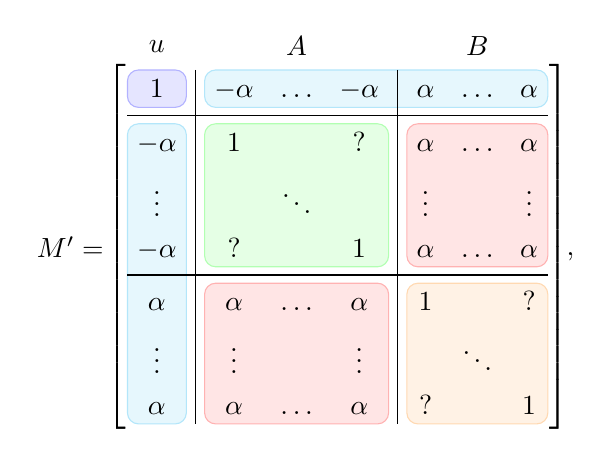
\begin{tikzpicture}[bmatrix, baseline]         
        \matrix (m) {
            1 &[4pt] -\alpha & \dots  &-\alpha &[4pt] \alpha & \dots & \alpha \\[4pt]
            -\alpha & 1 & \  & ? & \alpha & \dots & \alpha \\ 
            \vdots & \  & \ddots & \  & \vdots & \  & \vdots \\ 
            -\alpha & ? & \  & 1 & \alpha & \dots & \alpha \\[4pt] 
            \alpha & \alpha & \dots & \alpha & 1 & \  & ? \\ 
            \vdots &\vdots & \  &\vdots & \  & \ddots & \\ 
            \alpha & \alpha & \dots & \alpha & ? & \  & 1  \\
        };

        \coordinate (c1-w) at (m-2-1.west);
        \coordinate (c1-e) at ($(m-2-1.east) + (0, 0.1)$);
        \coordinate (c2-w) at (m-1-2.west);
        \coordinate (c2-e) at (m-1-4.east);
        \coordinate (c3-w) at (m-2-5.west);
        \coordinate (c3-e) at (m-2-7.east);
        \coordinate (mc1) at ($(c1-e)!.5!(c2-w)$);
        \coordinate (mc2) at ($(c2-e)!.5!(c3-w)$);

        \coordinate (r1-n) at (m-1-1.north);
        \coordinate (r1-s) at (m-1-1.south);
        \coordinate (r2-n) at (m-2-2.north);
        \coordinate (r2-s) at (m-4-2.south);
        \coordinate (r3-n) at (m-5-5.north);
        \coordinate (r3-s) at (m-7-7.south);
        \coordinate (mr1) at ($(r1-s)!.5!(r2-n)$);
        \coordinate (mr2) at ($(r2-s)!.5!(r3-n)$);

        \begin{scope}[on background layer]
            \draw[fill=blue!10, draw=blue!30, rounded corners] (r1-n -| c1-w) rectangle (r1-s -| c1-e);
            \draw[fill=red!10, draw=red!30, rounded corners] (r3-n -| c2-w) rectangle (r3-s -| c2-e);
            \draw[fill=red!10, draw=red!30, rounded corners] (r2-n -| c3-w) rectangle (r2-s -| c3-e);
            \draw[fill=orange!10, draw=orange!30, rounded corners] (r3-n -| c3-w) rectangle (r3-s -| c3-e);
            \draw[fill=green!10, draw=green!30, rounded corners] (r2-n -| c2-w) rectangle (r2-s -| c2-e);
            \draw[fill=cyan!10, draw=cyan!30, rounded corners] (r1-n -| c2-w) rectangle (r1-s -| c3-e);
            \draw[fill=cyan!10, draw=cyan!30, rounded corners] (r2-n -| c1-w) rectangle (r3-s -| c1-e);
        \end{scope}
        
        \draw[-] (r1-n -| mc1) -- (r3-s -| mc1);
        \draw[-] (r1-n -| mc2) -- (r3-s -| mc2);
        \draw[-] (mr1 -| c1-w) -- (mr1 -| c3-e);
        \draw[-] (mr2 -| c1-w) -- (mr2 -| c3-e);

        \node (label) at ($(m-1-1.north west)!.5!(m-7-1.south west) - (0.875, 0)$) {$M' = $};
        \node (comma) at ($(m-1-7.north east)!.52!(m-7-7.south east) + (0.3, 0)$) {,};
        \node (u) at ($(r1-n) + (0, 0.3)$) {$u$};
        \node (B) at ($(r1-n -| m-1-3.north) + (0, 0.3)$) {$A$};
        \node (A) at ($(r1-n -| m-1-6.north) + (0, 0.3)$) {$B$};
    \end{tikzpicture}
\end{document}